\chapter{Исследовательская часть}

\section{Интерфейс приложения}

На рисункaх  \ref{fig:интерфейс} -- \ref{fig:работа} приведено изображение интерфейса главного экрана приложения.

\begin{figure}[h!]
	\centering{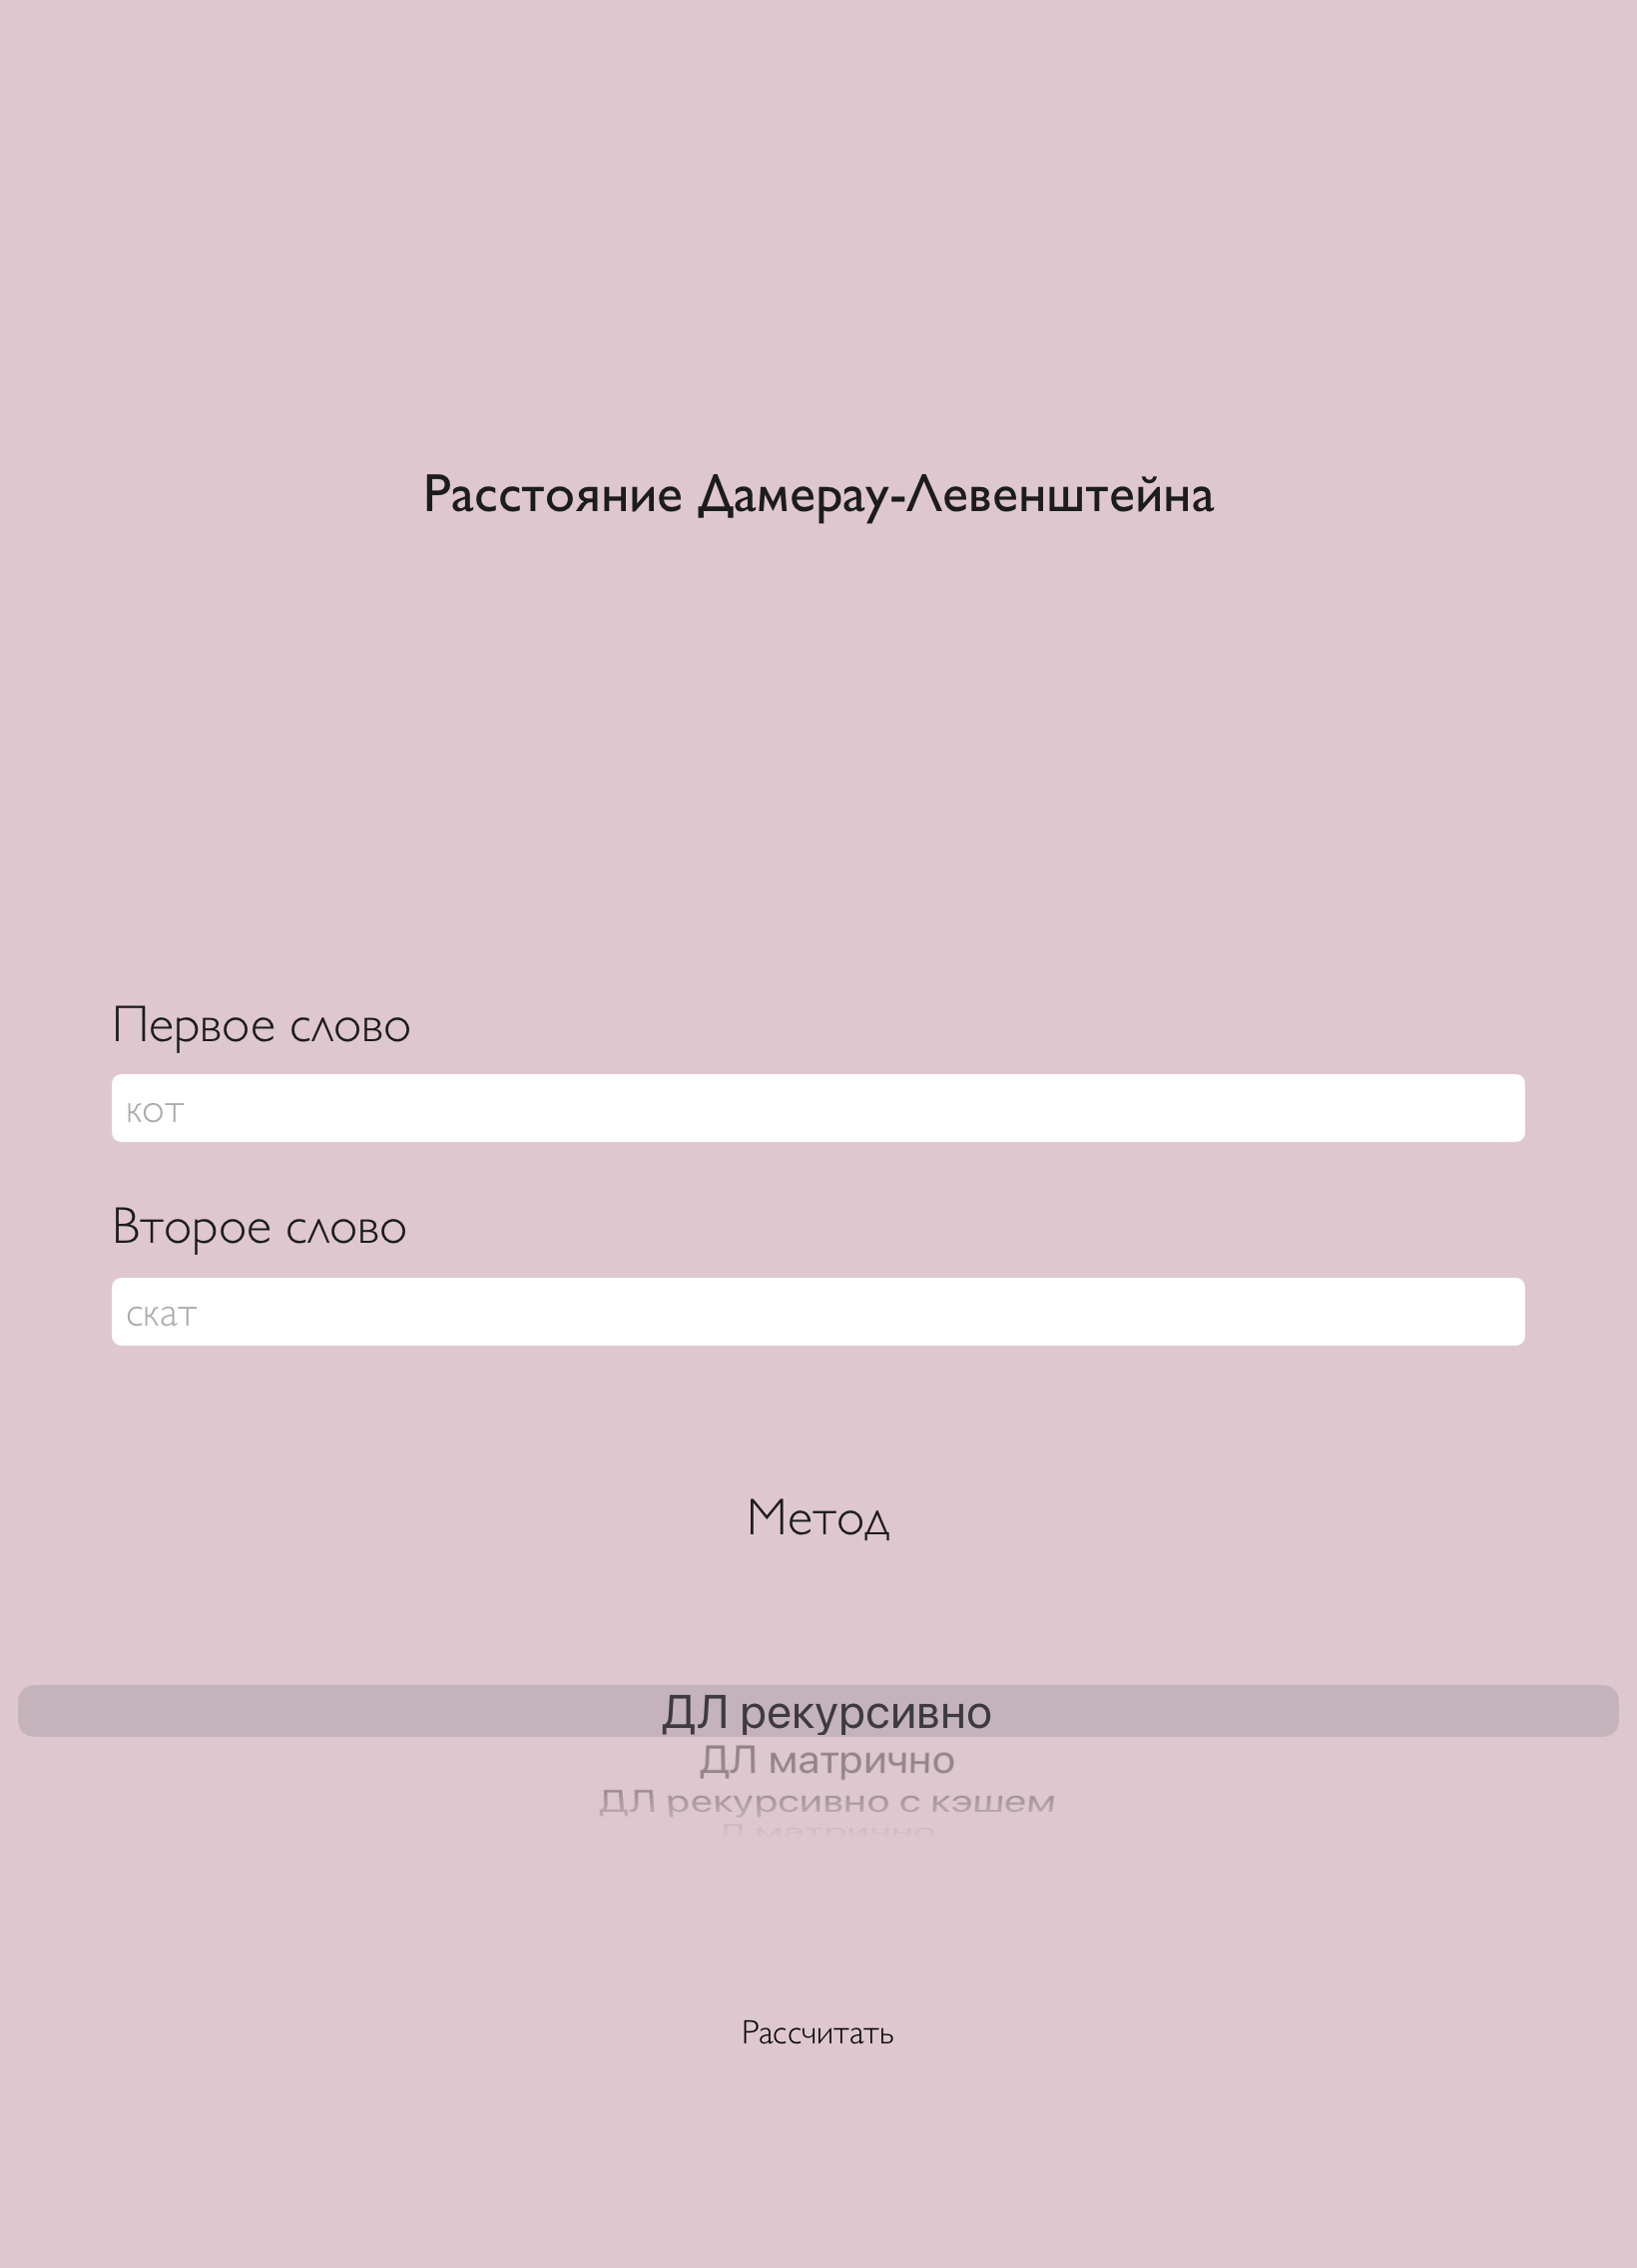
\includegraphics[scale=0.28]{img/интерфейс.jpg}}
	\caption{Интерфейс}
	\label{fig:интерфейс}
\end{figure}


Главный экран приложения дает возможность ввести две строки -- слова, для которых будет вычисляться расстояние, а также выбрать метод, с помощью которого оно будет найдено. При нажатии на кнопку <<Рассчитать>>, появляется второй экран, отображающий график зависимости времени (в секундах) от количества произведенных операций и результирующее расстояние.

\begin{figure}[h!]
	\centering{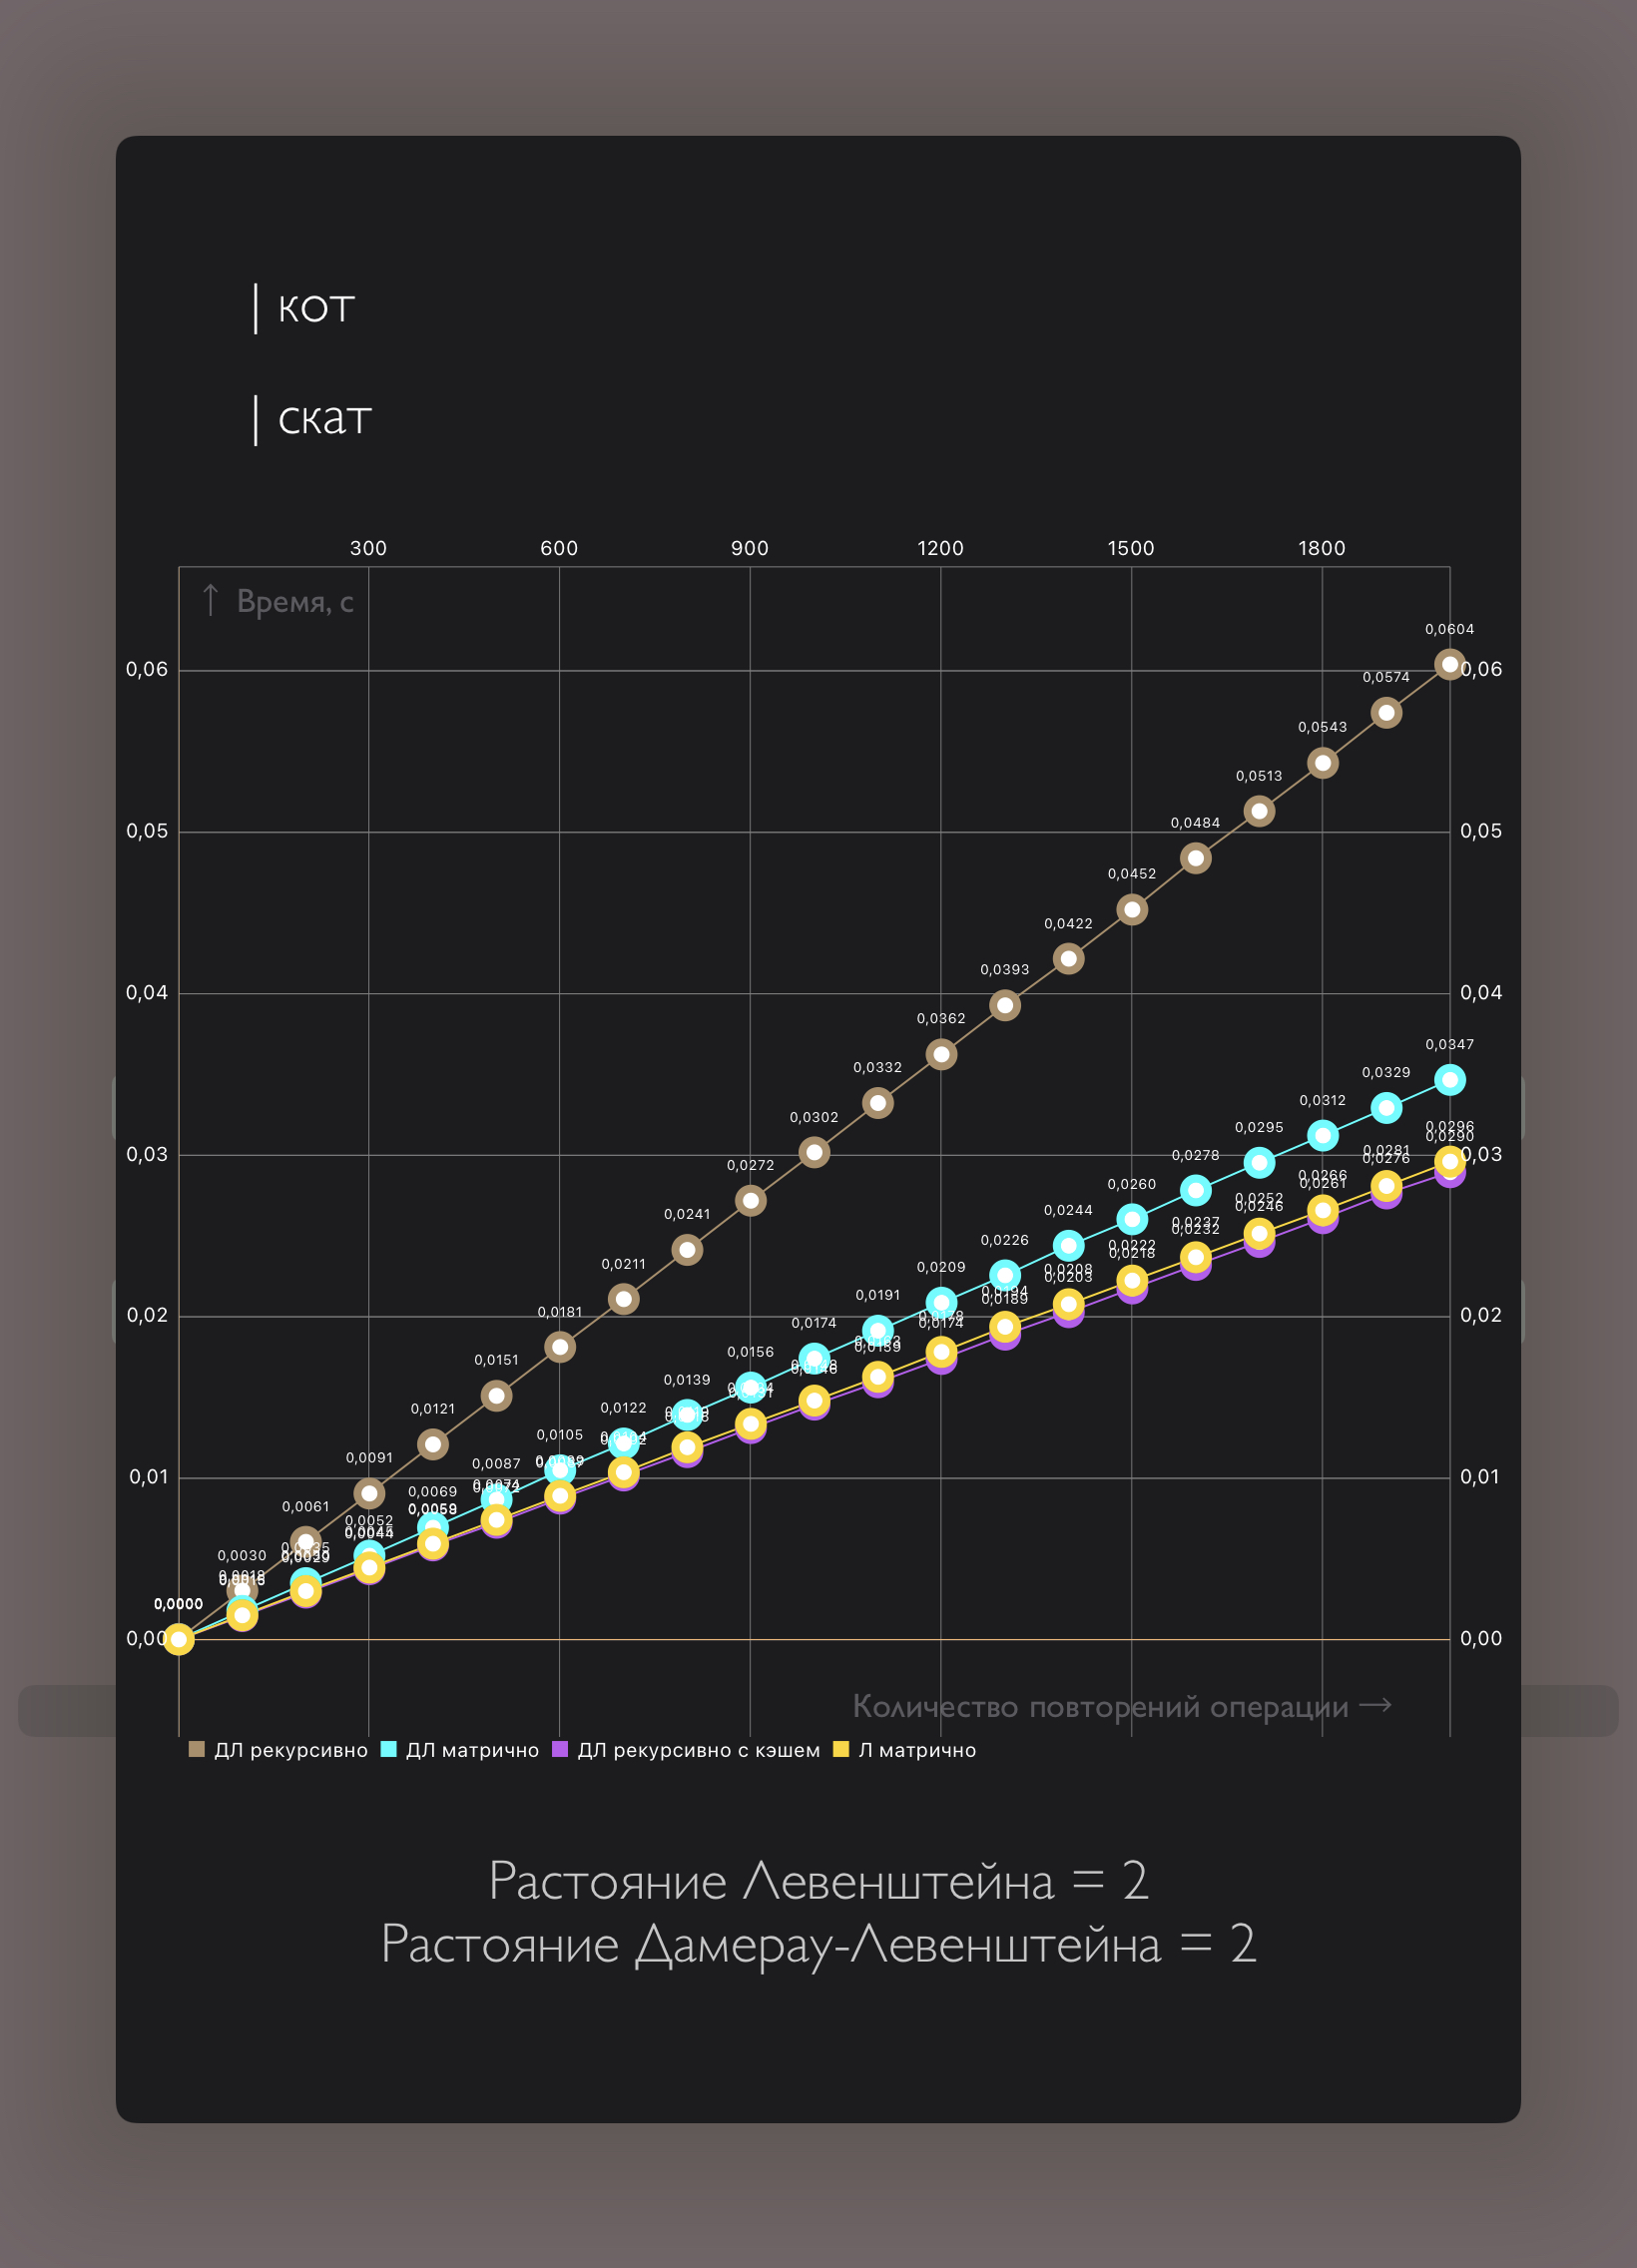
\includegraphics[scale=0.28]{img/работа.jpg}}
	\caption{Экран с результатом}
	\label{fig:работа}
\end{figure}

\section{Технические характеристики}

Технические характеристики устройства, на котором выполнялось тестирование:

\begin{itemize}
	\item операционная система: iOS 14.5;
	\item оперативная память: 4 Гб;
	\item процессор: Apple A14 Bionic 2990 МГц \cite{ipad};
\end{itemize}

Во время тестирования iPad не был подключен к другим устройствам и был включен в сеть питания.

\section{Время выполнения реализаций алгоритмов}

Все реализации алгоритмов сравнивались на строках длиной от 1 до 10 с шагом 100 в диапазоне повторений операций от 1 до 2000. 
 
На рисунках \ref{fig:короткое} --  \ref{fig:кенгуру_матрица} представлены результаты выполнения алгоритмов для строк <<a>> и <<б>>, <<кот>> и <<скат>>, <<кенгуру>> и <<кентавр>>.  
 
На рисунке \ref{fig:короткое} приведены результаты сравнения времени работы всех реализаций для слов малой длины, \ref{fig:среднее} -- результаты сравнения времени работы всех реализаций для слов средней длины, \ref{fig:длинное} -- результаты сравнения времени работы всех реализаций для слов большой длины. 

\begin{figure}[h!]
	\centering{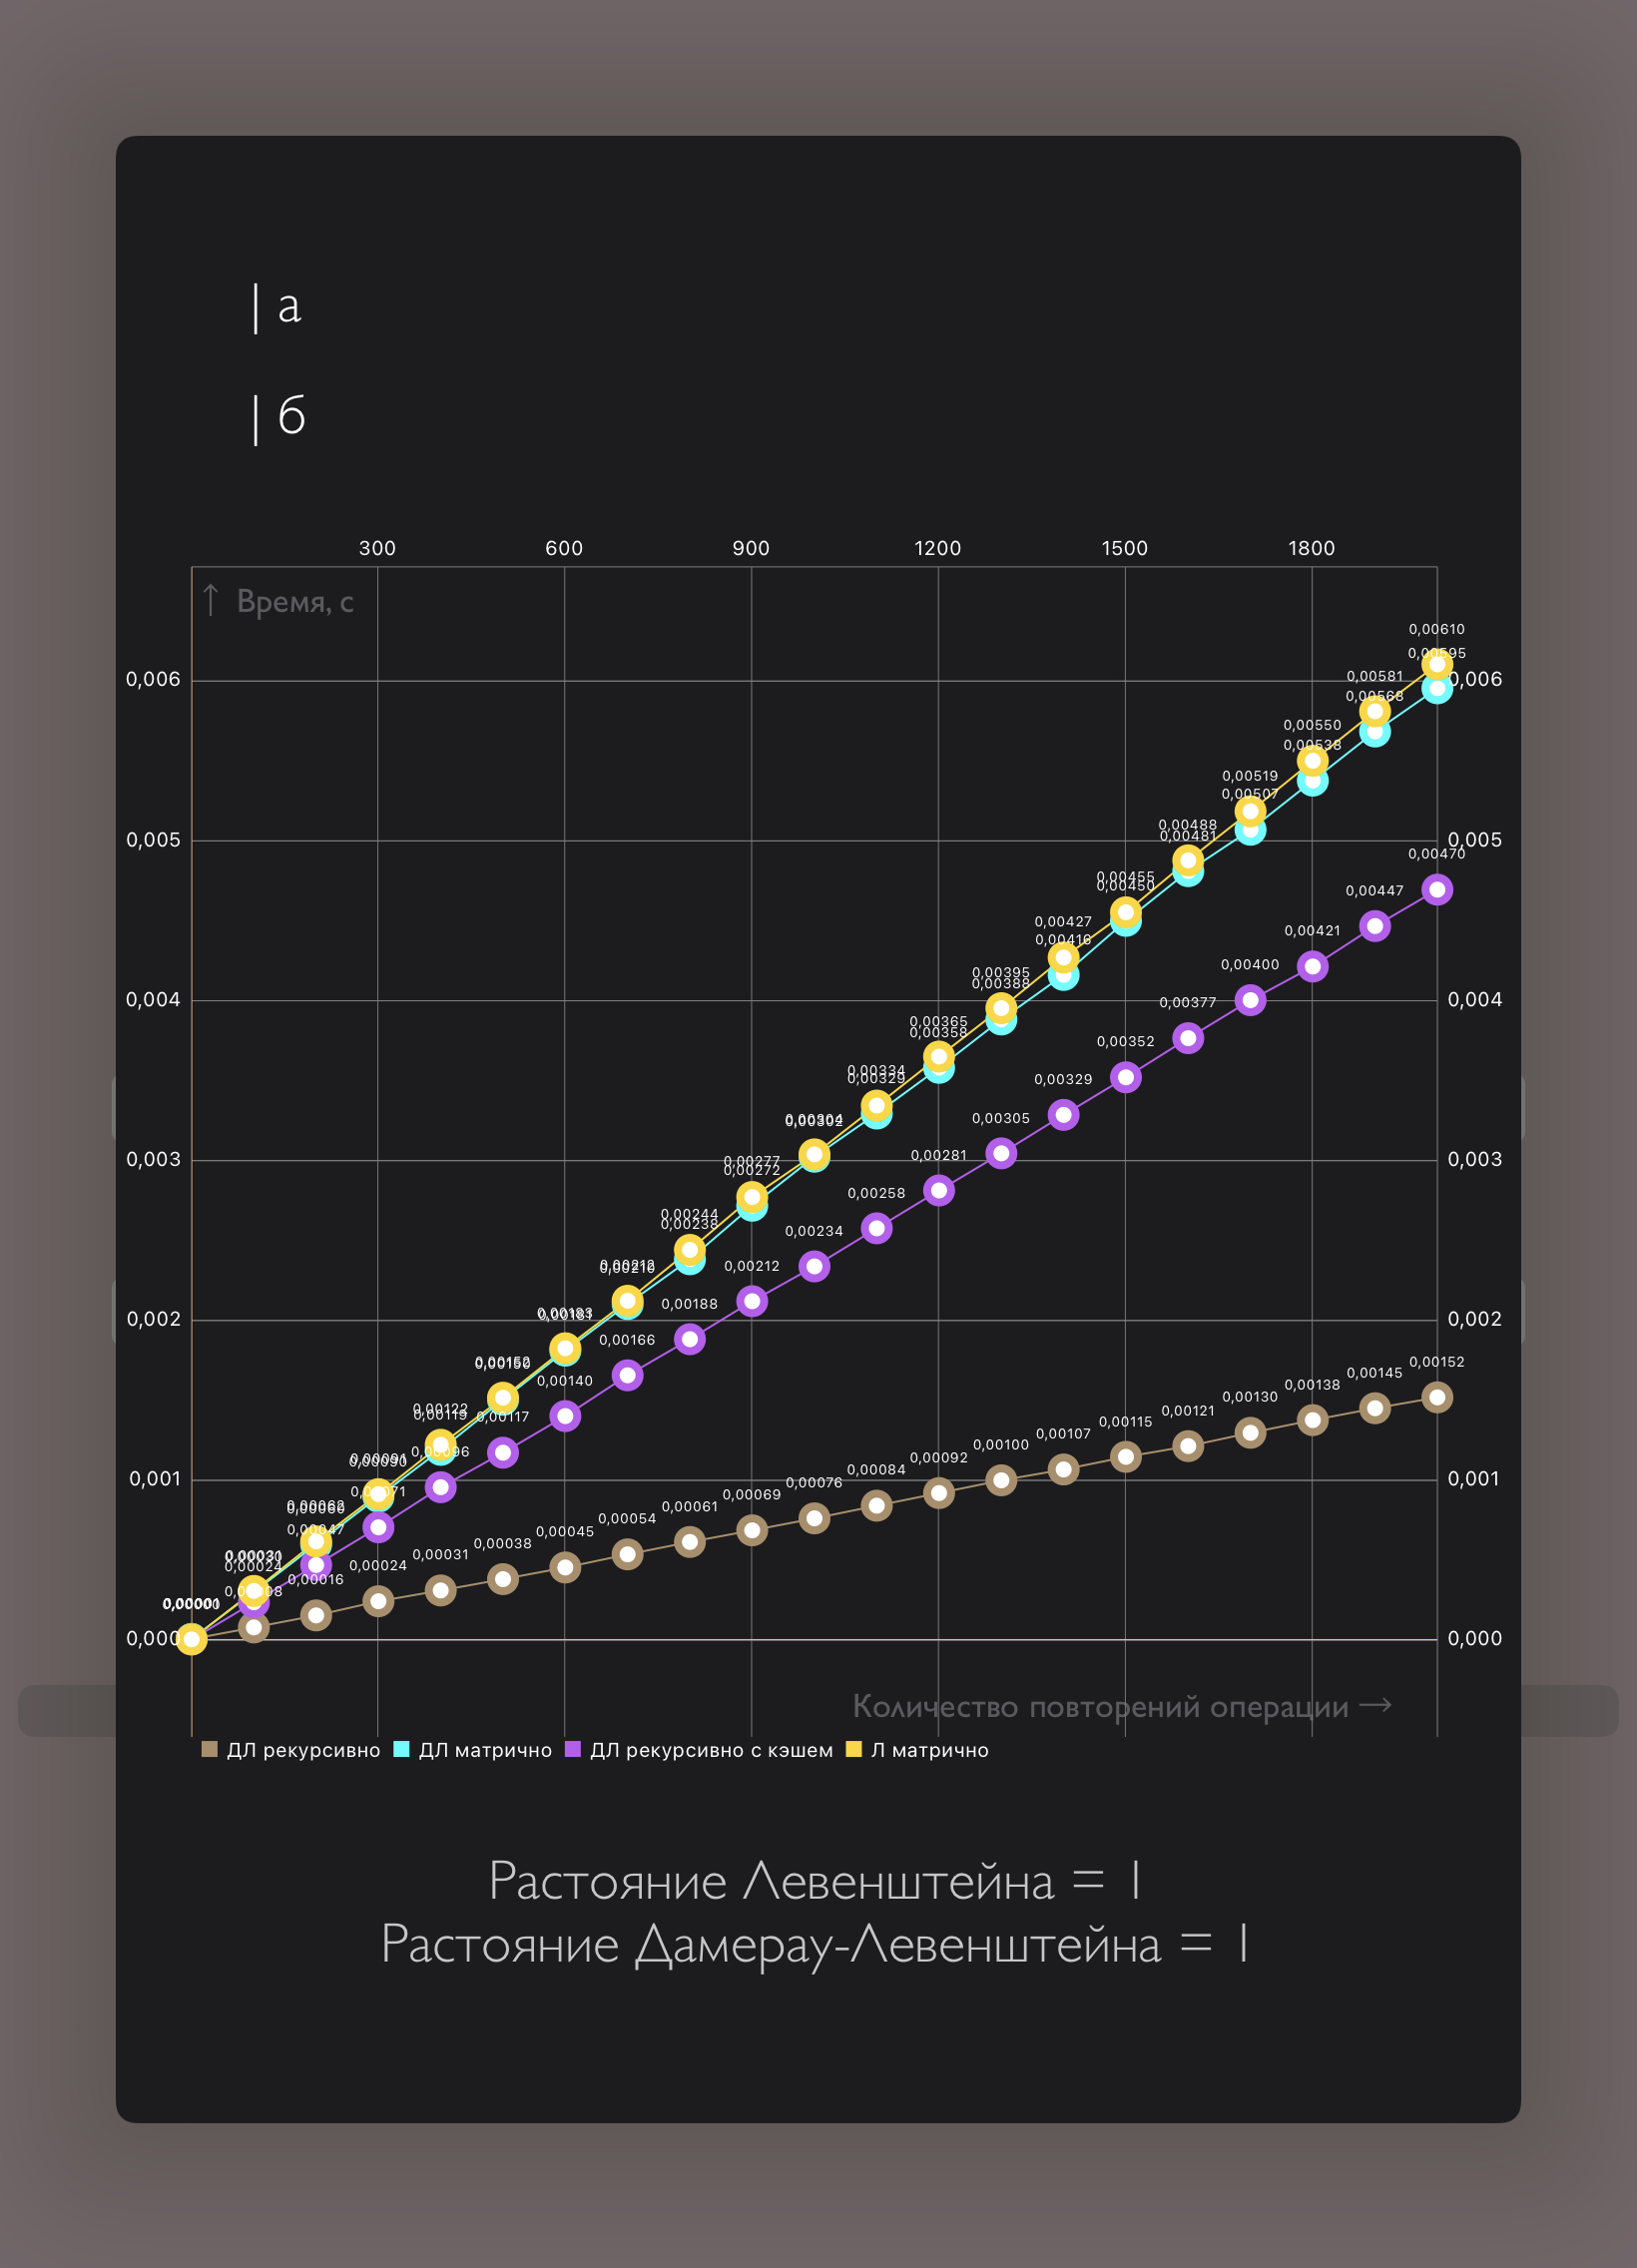
\includegraphics[scale=0.28]{img/короткое.jpg}}
	\caption{Сравнение времени работы реализаций алгоритмов при малой длине слов (1-2 символa)}
	\label{fig:короткое}
\end{figure}

\begin{figure}[h!]
	\centering{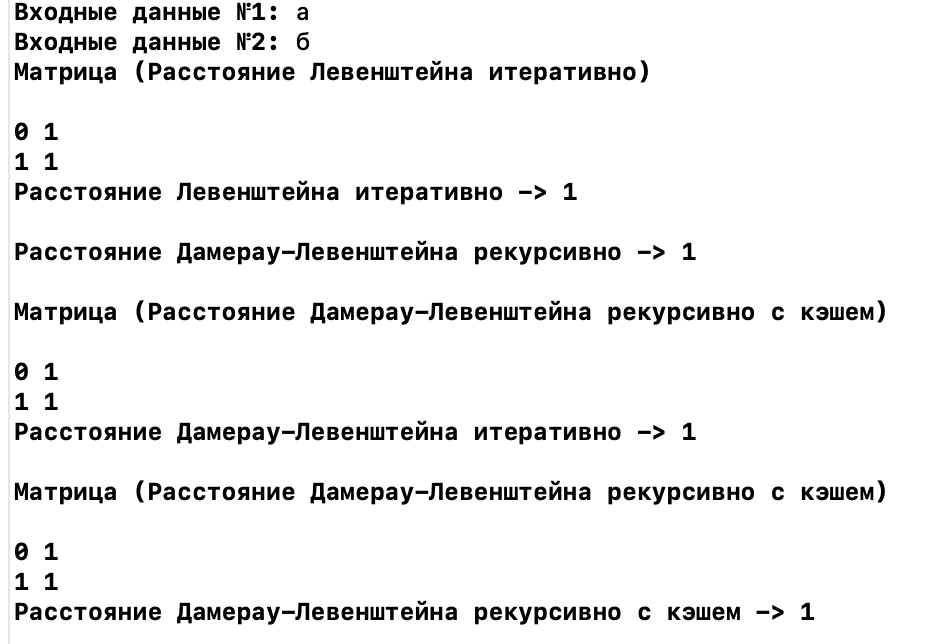
\includegraphics[scale=0.9]{img/аб_матрица.png}}
	\caption{Матрицы алгоритмов при малой длине слов (1-2 символa)}
	\label{fig:аб_матрица}
\end{figure}

\begin{figure}[h!]
	\centering{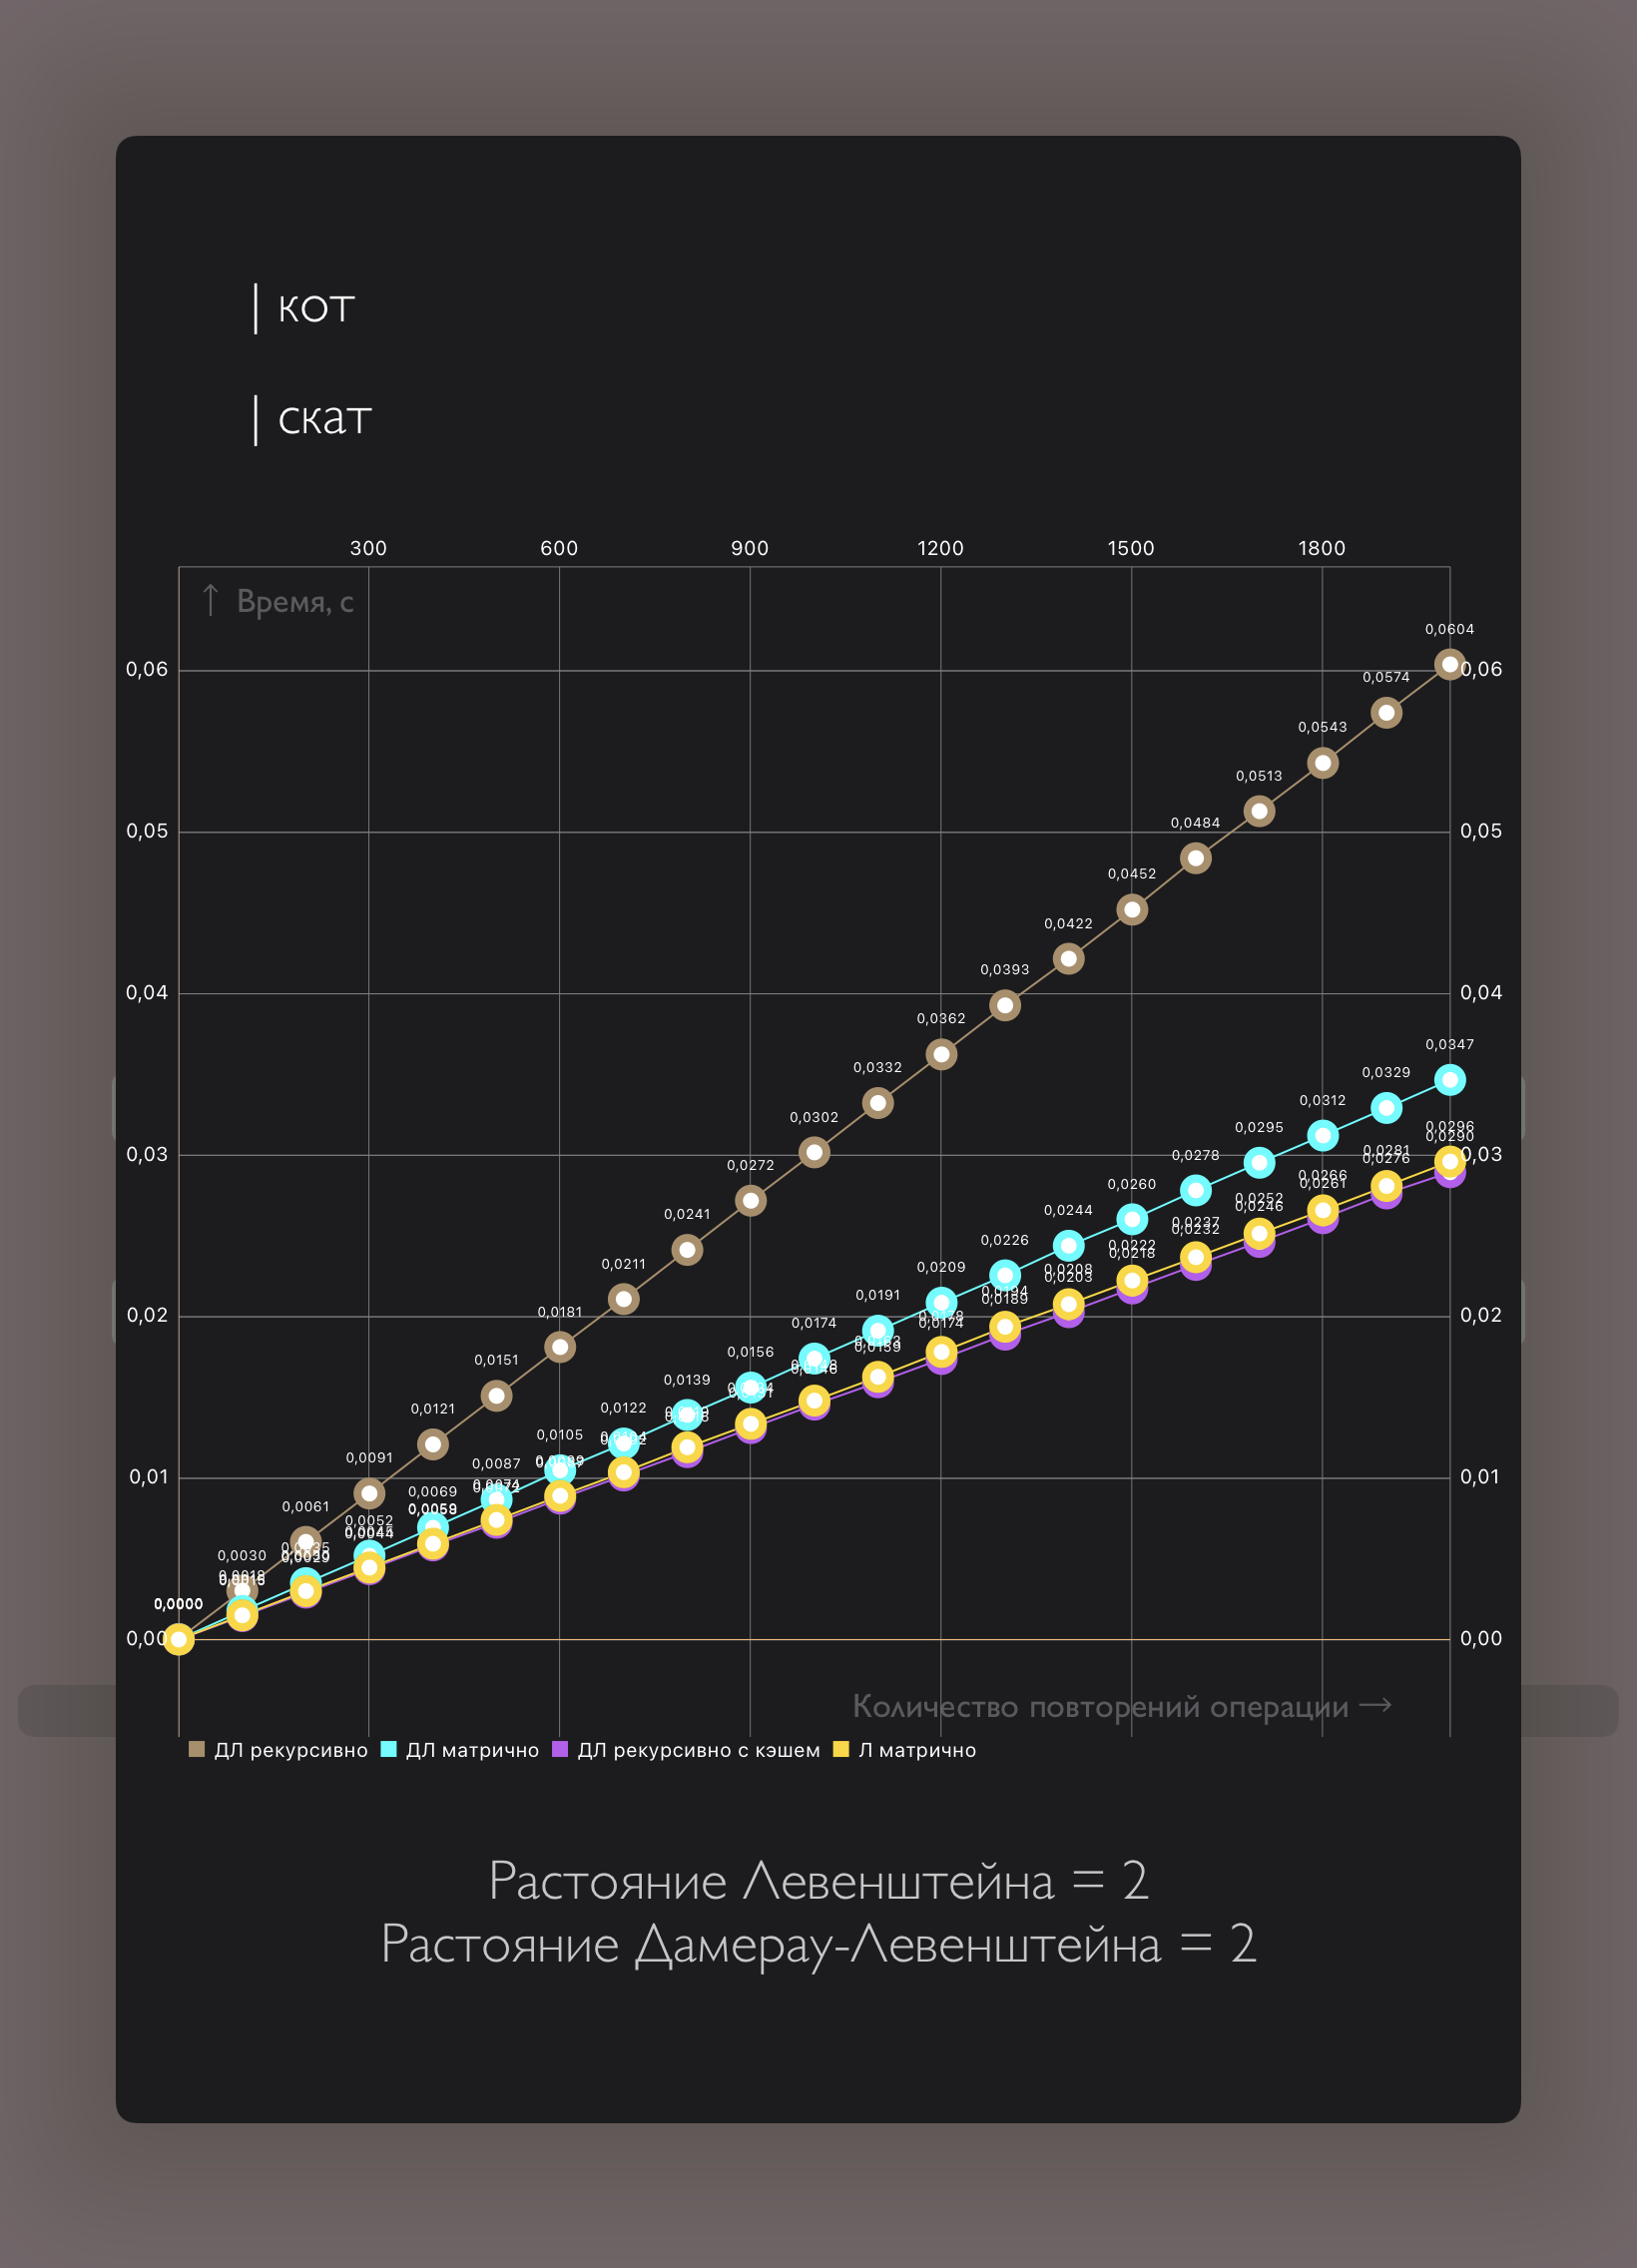
\includegraphics[scale=0.28]{img/среднее.jpg}}
	\caption{Сравнение времени работы реализаций алгоритмов при средней длине слов (3-6 символов)}
	\label{fig:среднее}
\end{figure}

\begin{figure}[h!]
	\centering{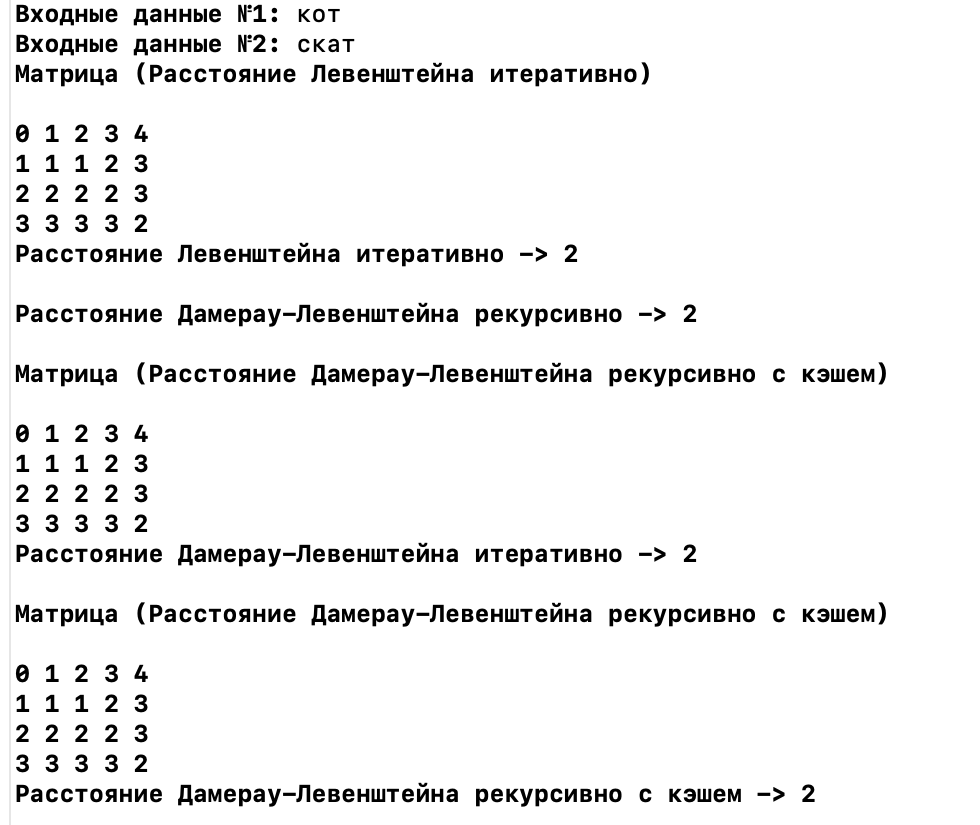
\includegraphics[scale=0.9]{img/котскат_матрица.png}}
	\caption{Матрицы алгоритмов при средней длине слов (3-6 символов)}
	\label{fig:котскат_матрица}
\end{figure}

\begin{figure}[h!]
	\centering{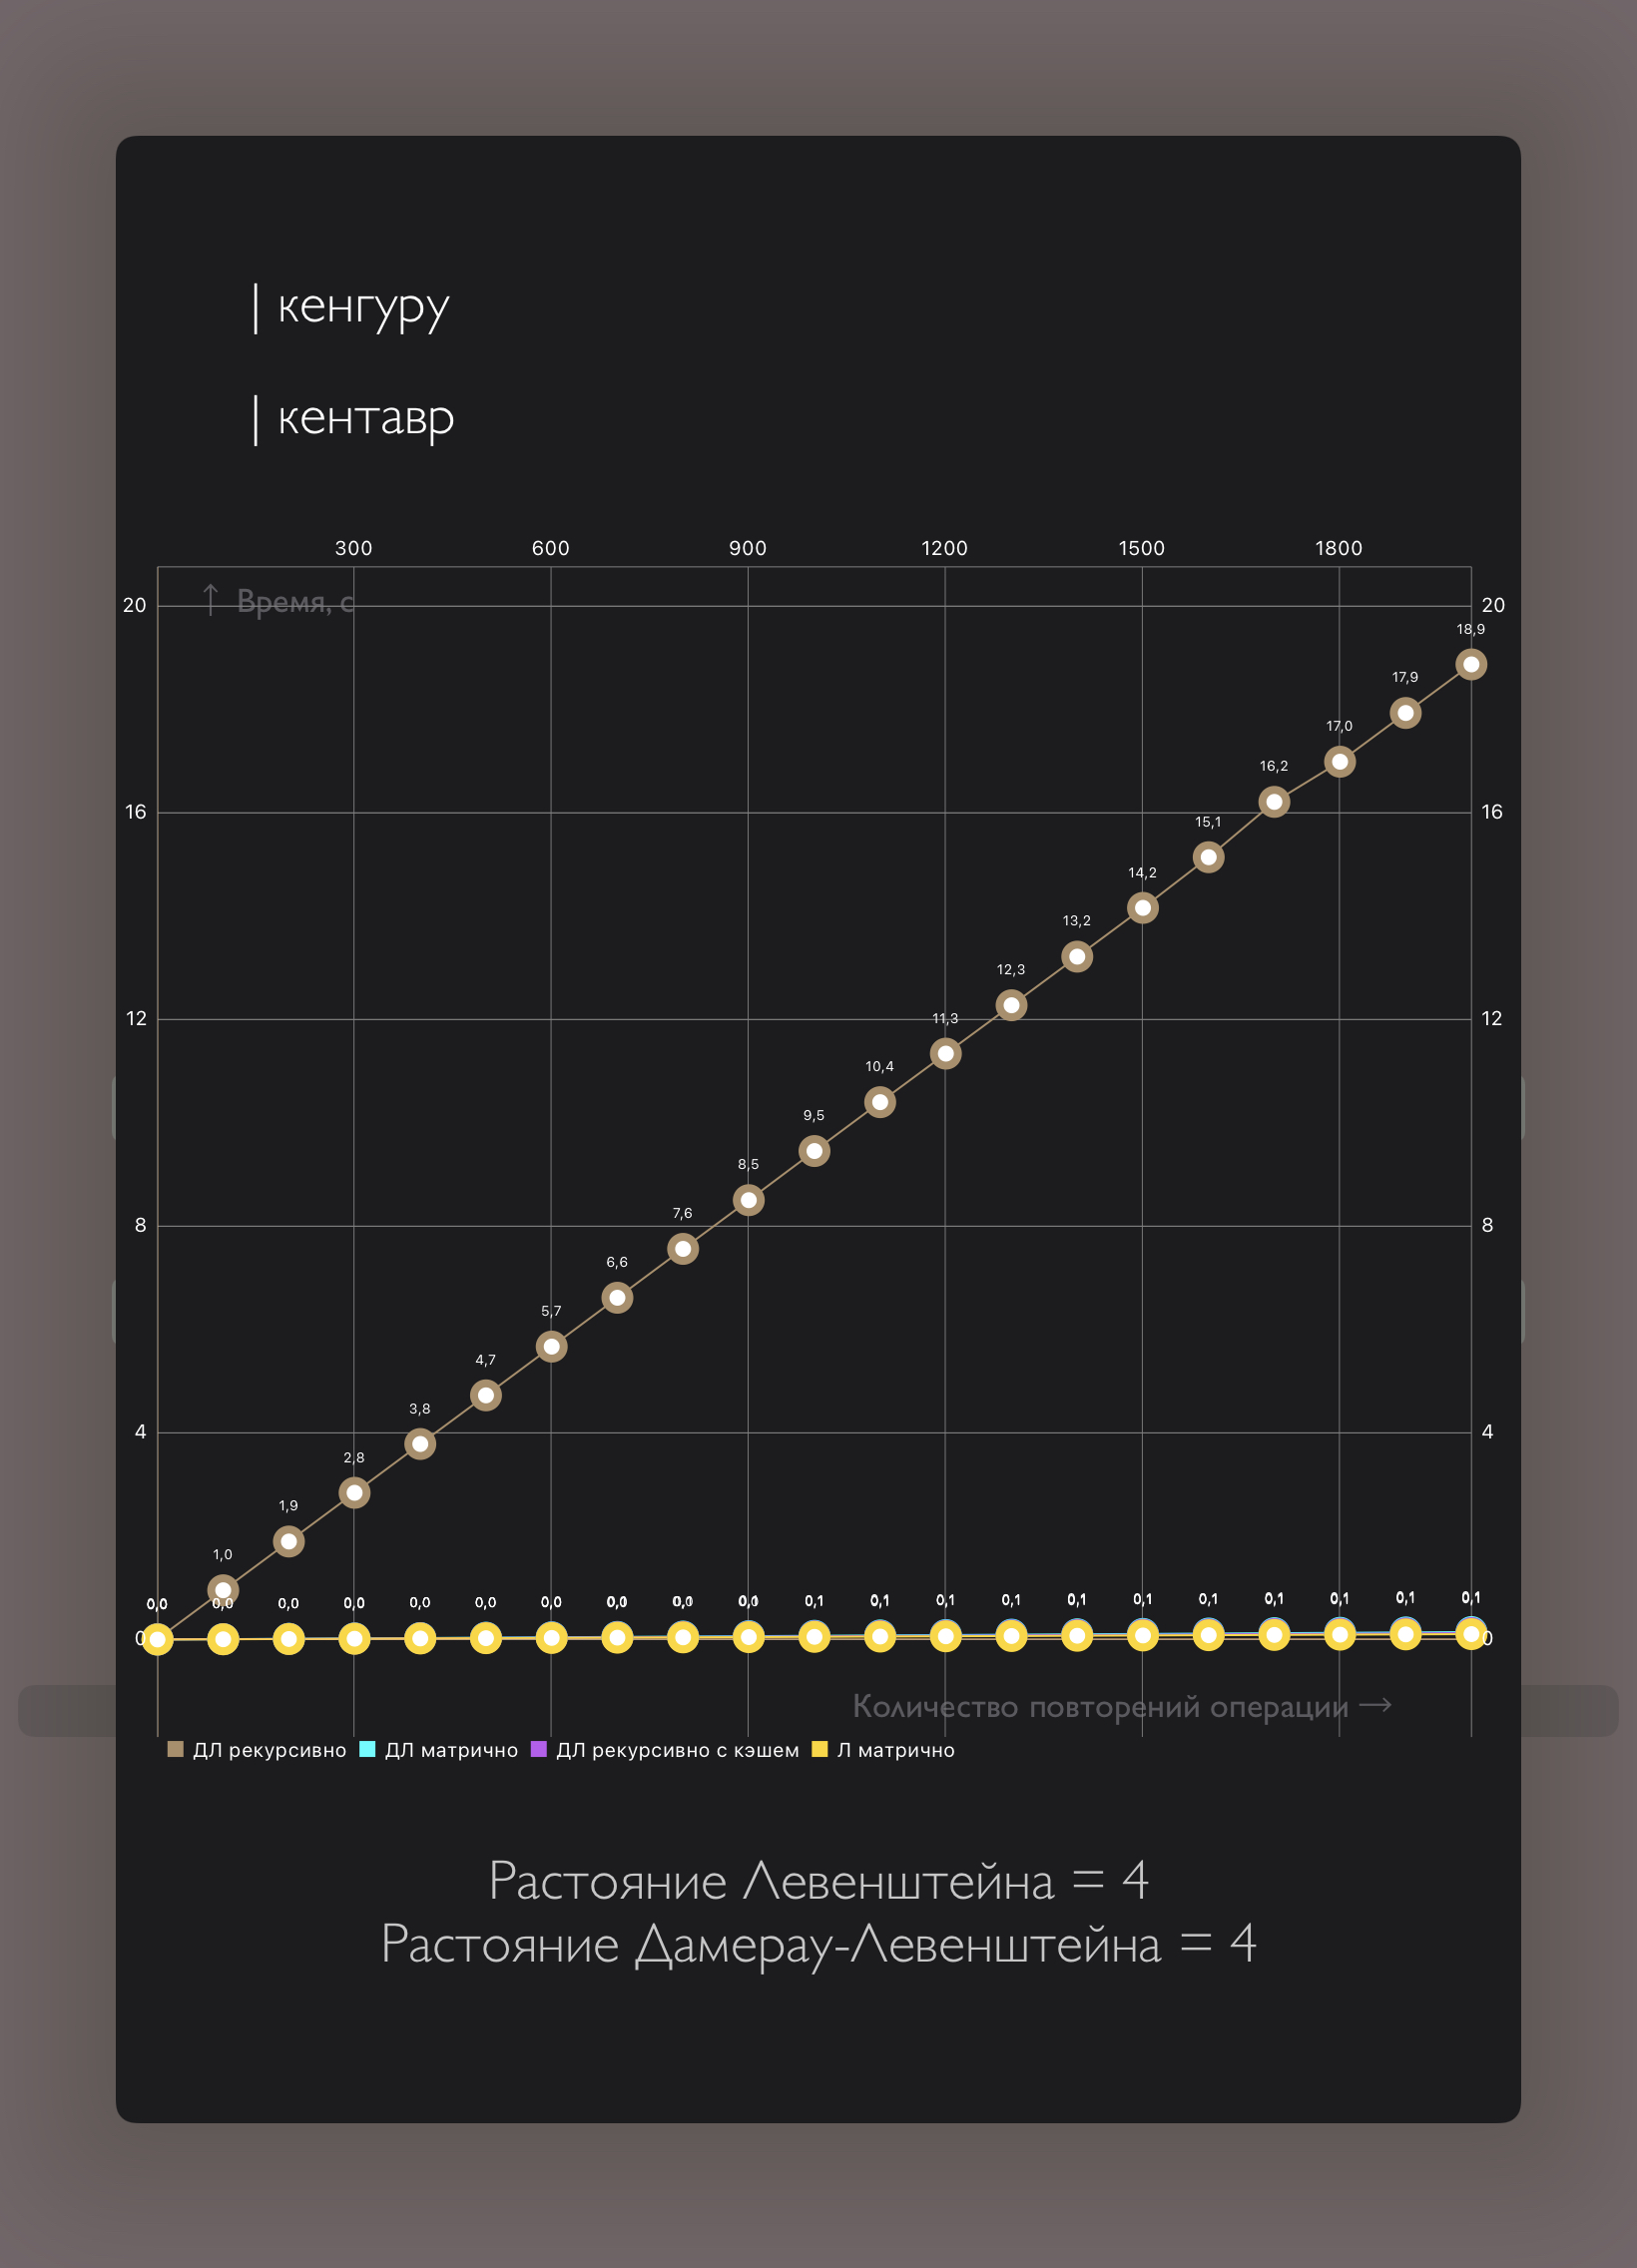
\includegraphics[scale=0.28]{img/длинное.jpg}}
	\caption{Сравнение времени работы реализаций алгоритмов при большой длине слов (7-10 символов)}
	\label{fig:длинное}
\end{figure}

\begin{figure}[h!]
	\centering{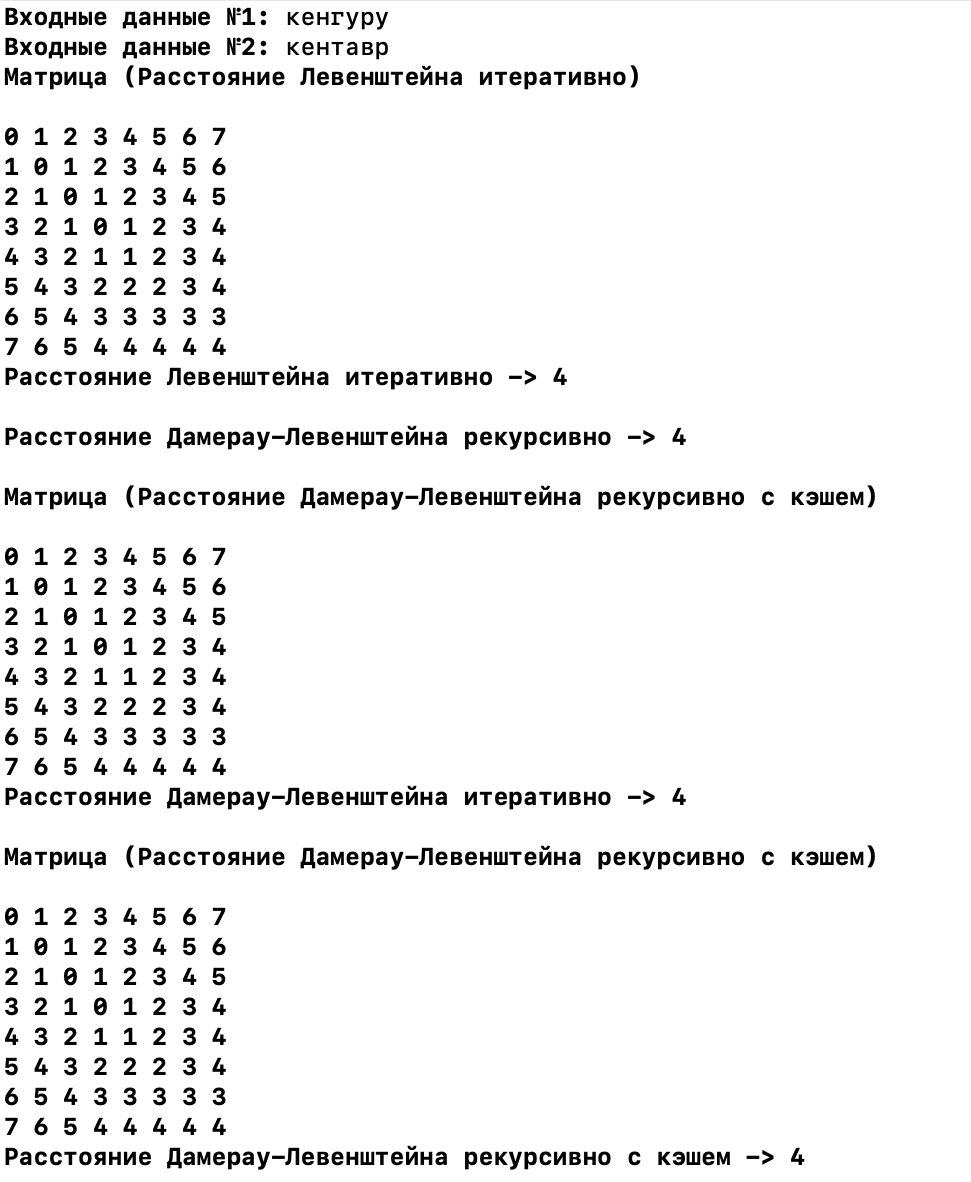
\includegraphics[scale=0.9]{img/кенгуру_матрица.png}}
	\caption{Матрицы алгоритмов при при большой длине слов (7-10 символов)}
	\label{fig:кенгуру_матрица}
\end{figure}

При малой длине слов эффективнее всего использовать рекурсивный метод без кэша, а при средней и большой длине слов более рационально использование матричного алгоритма: рекурсивный алгоритм в данном случае проигрывает по времени. Причем при наибольшей рассматриваемой длине слов -- в разы. Также можно отметить, что при малой длине слов алгоритм Левенштейна проигрывает по времени реализациям Дамерау-Левенштейна. Однако при увеличении длины слов уступает только рекурсивному алгоритму, использующему кэш. 


\section{Используемая память}

Алгоритмы нахождения расстояния Левенштейна и Дамерау-Левенштейна не отличаются друг от друга с точки зрения использования памяти.

Пусть длина строки S1 - n, длина строки S2 - m, тогда затраты памяти для рекурсивного и итеративного алгоритмов будут следующими:
\begin{itemize}
\item матричный алгоритм Левенштейна:\begin{itemize}
	\item строки S1, S2 -- $(m + n) \cdot MemoryLayout<Character>.size$
	\item матрица -- $((m + 1) \cdot (n + 1)) \cdot MemoryLayout<Int>.size$
	\item текущая строка матрицы -- $(n + 1) \cdot MemoryLayout<Int>.size$
	\item длины строк -- $2 \cdot MemoryLayout<Int>.size$
	\item вспомогательные переменные -- $3 \cdot MemoryLayout<Int>.size$
	\end{itemize}

\item рекурсивный алгоритм Дамерау-Левенштейна (для каждого вызова):\begin{itemize}
	\item строки S1, S2 -- $(m + n) \cdot MemoryLayout<Character>.size$
	\item длины строк -- $2 \cdot MemoryLayout<Int>.size$
	\item вспомогательные переменные -- $4 \cdot MemoryLayout<Int>.size$
	\item адрес возврата
	\end{itemize}
\end{itemize}

Существенной является разница затрат памяти, используемой для хранения матрицы в итеративном алгоритме, и памяти, используемой для хранения строки в рекурсивном алгоритме. Очевидно, что произведение длин строк требует больших затрат по памяти, нежели сумма. При этом память, затрачиваемая на хранение вспомогательных переменных, длин строк и прочего, не играет ключевой роли. 

\section*{Вывод}


Рекурсивные реализации алгоритмов нахождения расстояний Левенштейна и Дамерау-Левенштейна, не использующие кэширование, работают на порядок дольше итеративных реализаций. При применении кэширования они требуют меньше времени, однако все равно уступают по производительности итеративным алгоритмам, особенно при большой длине строк. 

Но по расходу памяти итеративные реализации проигрывают рекурсивным: максимальный размер используемой памяти в них пропорционален произведению длин строк, в то время как в рекурсивных — сумме длин строк.

Если же применить к итеративным реализациям оптимизацию по памяти, то они будут выигрывать как по затрачиваемой памяти, так и по времени выполнения.
